% =========================================================================
% 文件路径: tex/demo/main.tex
% 用途: 全面集成测试 (Chinese + Math + Fonts + Graphics + Bibliography)
% =========================================================================

% [Group 2 测试] 强行指定 Fandol 字体,兼容 Windows Server 环境
\PassOptionsToPackage{fontset=fandol}{ctex}

% [Group 4 测试] 加载 elegantpaper 模板 (依赖 kvoptions, etoolbox 等)
% [Group 5 测试] bibend=bibtex 测试 biblatex 的后端支持
\documentclass[lang=cn, chinesefont=ctexfont, bibend=bibtex]{elegantpaper}

% [Group 5 测试] 加载常用功能包
\usepackage{custom}       % 用户自定义样式
\usepackage{tikz}         % 绘图测试 (依赖 pgf)
\usepackage{mwe}          % 占位图测试 (依赖 mwe)
\usepackage{listings}     % 代码高亮测试
\usepackage{array}        % 表格测试 (依赖 tools)

% =========================================================================
% 0. 自动生成测试用参考文献 (.bib)
% =========================================================================
\begin{filecontents}[overwrite]{ref.bib}
@article{test-en,
  title   = {TinyTeX: A lightweight LaTeX distribution},
  author  = {Xie, Yihui},
  journal = {TUGboat},
  year    = {2019}
}
@book{test-cn,
  title     = {LaTeX 自动化测试指南},
  author    = {GitHub Actions},
  publisher = {开源出版社},
  year      = {2025},
  address   = {云端}
}
\end{filecontents}
\addbibresource{ref.bib}

% =========================================================================
% 文档信息
% =========================================================================
\title{TinyTeX 模块化环境全量测试报告}
\author{CI/CD Bot}
\date{\zhtoday}

\begin{document}

\maketitle

\begin{abstract}
    本文档用于验证 \texttt{install-tinytex.ps1} 脚本中定义的 5 个安装组是否工作正常。测试点涵盖:中文 Fandol 字体、数学公式字体、TikZ 矢量绘图、智能图片加载、复杂表格以及参考文献生成。
    \keywords{自动化测试; 模块化安装; LaTeX}
\end{abstract}

% =========================================================================
% [Group 2 & 3 测试] 中文与字体
% =========================================================================
\section{中文与字体支持 (Group 2 \& 3)}
\begin{itemize}
    \item \textbf{中文字体}:这是一段中文测试。如果显示正常,说明 \texttt{ctex} 和 \texttt{fandol} 字体包工作正常。
    \item \textbf{数字转换}:\texttt{zhnumber} 测试 -> 123 转换为:\zhnumber{123}。
    \item \textbf{英文字体}:This text checks \texttt{tex-gyre} fonts (Termes/Heros).
\end{itemize}

% =========================================================================
% [Group 3 测试] 数学公式
% =========================================================================
\section{数学与特殊符号 (Group 3)}
测试 \texttt{newtx} 数学字体和 \texttt{esint} 扩展符号:
\begin{equation}
    \oint_{\partial V} \mathbf{E} \cdot d\mathbf{l} = -\frac{d}{dt} \iint_S \mathbf{B} \cdot d\mathbf{S}
\end{equation}
如果积分号显示正常,说明 Group 3 安装成功。

% =========================================================================
% [Group 5 测试] 图片与绘图
% =========================================================================
\section{图形与多媒体 (Group 5)}

\subsection{智能缺省图测试 (mwe)}
调用 \texttt{example-image},测试 \texttt{mwe} 包是否安装:
\begin{figure}[htbp]
    \centering
    \includegraphics[width=0.4\textwidth]{example-image-a} 
    \caption{标准测试图 A (依赖 mwe 包)}
\end{figure}

\subsection{TikZ 矢量绘图 (pgf)}
测试 \texttt{pgf} 底层库是否正常:
\begin{figure}[htbp]
    \centering
    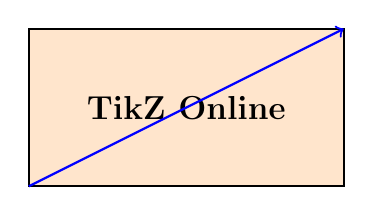
\begin{tikzpicture}
        \draw[fill=orange!20, thick] (0,0) rectangle (4,2);
        \node at (2,1) {\large \textbf{TikZ Online}};
        \draw[->, blue, thick] (0,0) -- (4,2);
    \end{tikzpicture}
    \caption{TikZ 绘图测试}
\end{figure}

% =========================================================================
% [Group 5 测试] 复杂表格
% =========================================================================
\section{复杂表格 (Group 5)}
测试 \texttt{booktabs} (三线表)、\texttt{multirow} 和 \texttt{makecell}:

\begin{table}[htbp]
    \centering
    \caption{宏包功能覆盖表}
    \begin{tabular}{llc}
        \toprule
        \textbf{安装组} & \textbf{关键宏包} & \textbf{状态} \\
        \midrule
        Group 1 & latexmk, tools & \makecell[c]{Ready} \\
        Group 2 & ctex, fandol   & \makecell[c]{Ready} \\
        Group 3 & newtx, amsmath & \multirow{2}{*}{Checked} \\
        Group 4 & footmisc, appendix & \\
        \bottomrule
    \end{tabular}
\end{table}

% =========================================================================
% [Group 4 & 5 测试] 引用、脚注与附录
% =========================================================================
\section{其他功能测试 (Group 4 \& 5)}

\subsection{参考文献 (biblatex + bibtex)}
这里测试引用功能\cite{test-en}。以及中文引用支持\cite{test-cn}。如果此处显示数字且文末有列表,说明 \texttt{latexmk} 自动调用 \texttt{bibtex} 成功。

\subsection{脚注测试 (footmisc)}
这是一个正文文本\footnote{这是一个脚注,测试 footmisc 宏包是否造成 crash。}。

% 打印参考文献
\printbibliography[heading=bibintoc, title=参考文献]

% 附录测试 (appendix)
\appendix
\section{附录测试}
如果能看到这里,说明 \texttt{appendix} 宏包加载正常,没有触发 Emergency Stop。

\end{document}